
\hformbar

\newpage

\formdesc{Rappel Nyquist}

\begin{enumerate}
    \item Condition de stabilité en boucle fermée basée sur un critère en boucle ouverte !
    \item Outil important pour l‘analyse des systèmes réglés, marge de gain $A_m$ , marge de phase $\varphi_m$.
    \item Outil important pour la synthèse des systèmes réglés, choix de $K_p$ pour obtenir $\varphi_m$ souhaitée.
\end{enumerate}

$\varphi_m = arg(G_o(j\omega_{co}))- (-\pi)$ \quad [rad]

\vspace{3mm}

$A_{m,dB} = -|G_o(j\omega_{\pi})| $\quad  [dB]

\vspace{3mm}

\formtitle{Liens entre la boucle ouverte et la boucle fermée} 

bande passante à -3 dB en boucle fermée $\omega_{bp} \approx$ pulsation de coupure en boucle ouverte $\omega_{co}$

$\omega_{bande,passante} = \omega_{co}$

Pulsation de coupure en b.o. $\omega_{co} \Leftrightarrow $ rapidité en b.f

\hformbar

\formdesc{Compensation du pôle dominant}

\begin{enumerate}
    \item Améliorer la dynamique, c-à-d rendre la boucle fermée plus rapide
    \item Faciliter les calculs
\end{enumerate}

\formtitle{Zéros libres du régulateur PI, PD, PID} 


\vspace{2mm}

\underline{PI :}

\vspace{2mm}

{\noindent$G_c(s) = K_p \cfrac{1+T_i \cdot s}{T_i \cdot s} \rightarrow$}

\begin{wrapfigure}[2]{r}{0.25\textwidth}
    \begin{center}
        \vspace{-3.7cm}
        \begin{tikzpicture}[]
            \tikzmath{
            coordinate \x;
            \x1 = (-1.5,0);
            }
            \draw[->] (-2,0) -- (1,0) node [anchor=west] {$R$};
            \draw[->] (0,-0.5) -- (0,0.5) node [anchor=south] {$Img$};
            \draw[thick] (\x1) circle (4pt) node[above=0.2cm] {$Z = -\cfrac{1}{T_i}$};
        \end{tikzpicture}
    \end{center}
  \end{wrapfigure}

  \vspace{10mm}

\underline{PD :}

\vspace{2mm}

{\noindent$G_c(s) = K_p (1+T_d \cdot s) \rightarrow$}

\begin{wrapfigure}[2]{r}{0.25\textwidth}
    \begin{center}
        \vspace{-3.5cm}
        \begin{tikzpicture}[]
            \tikzmath{
            coordinate \x;
            \x1 = (-1.5,0);
            }
            \draw[->] (-2,0) -- (1,0) node [anchor=west] {$R$};
            \draw[->] (0,-0.5) -- (0,0.5) node [anchor=south] {$Img$};
            \draw[thick] (\x1) circle (4pt) node[above=0.2cm] {$Z = -\cfrac{1}{T_d}$};
        \end{tikzpicture}
    \end{center}
  \end{wrapfigure}

  \vspace{10mm}


\underline{PID :}

\vspace{2mm}

{\noindent$G_c(s) = K_p \cfrac{1+T_i \cdot s+T_i \cdot T_d \cdot s^2}{T_i \cdot s}$}

\vspace{2mm}

zéros réels si : $T_i > 4\cdot T_d$

    \begin{center}
        \tikzset{cross/.style={cross out, draw=black, minimum size=2*(#1-\pgflinewidth), inner sep=0pt, outer sep=0pt},
        cross/.default={4pt}}
        \begin{tikzpicture}[]
            \tikzmath{
            coordinate \x;
            \x1 = (-5,0);
            \x2 = (-2,0);
            \x3 = (0,0);
            }
            \draw[->] (-6,0) -- (1,0) node [anchor=west] {$R$};
            \draw[->] (0,-0.5) -- (0,0.5) node [anchor=south] {$Img$};
            \draw[thick] (\x3) node[cross] {};
            \draw[thick] (\x2) circle (4pt) node[above=0.2cm] {$Z_1 \approx -\cfrac{1}{T_i}$};
            \draw[thick] (\x1) circle (4pt) node[above=0.2cm] {$Z_2 \approx -\cfrac{1}{T_d}$};
        \end{tikzpicture}
    \end{center}

    La compensation se fait en appliquant la règle suivante : 
    
    Zéro du régulateur = Pôle de système à régler

    \tikzset{cross/.style={cross out, draw=black, minimum size=2*(#1-\pgflinewidth), inner sep=0pt, outer sep=0pt},
cross/.default={4pt}}

\tikzset{ % this style creates an arrow like the one you draw in the middle of a path
   ->-/.style={decoration={markings,mark=at position 0.5 with {\arrow{Straight Barb}}},
               postaction={decorate}}
}
%default radius will be 1pt. 
\begin{tikzpicture}[]
    \tikzmath{
    coordinate \x;
    \x1 = (-2,0);
    \x2 = (-1,0);
    \x3 = (-5,0);
    \x4 = (-3.5,0);
    \x5 = (-1,0);
    }
    \draw[->] (-6,0) -- (1,0) node [anchor=west] {$R$};
    \draw[->] (0,-0.5) -- (0,0.5) node [anchor=south] {$Img$};

    \draw[thick] (\x1) node[cross] {};
    \draw[] (\x1) node[above=0.2cm] {$S_{a2}$};
    \draw[thick] (\x2) node[cross] {};
    \draw[] (\x2) node[above=0.2cm] {$S_{a1}$};
    \draw[thick] (\x4) node[cross] {};
    \draw[] (\x4) node[above=0.2cm] {$S_{a3}$};

    \draw[thick] (\x3) circle (4pt) node[above=0.2cm] {$Z_{a1} $};

    \draw[thick] (\x5) circle (4pt) node[below=0.2cm] {$Z_{c1} $};
    
\end{tikzpicture}


\hformbar

\newpage

\formdesc{schéma et FTZ dérivateur}


\begin{center}
    \begin{tikzpicture}[scale=0.5]
            \bXInput{E}
            \bXBloc[4]{sys}{$\cfrac{d}{dt}$}{E}
            \bXLink[$u(t)$]{E}{sys}
            \bXOutput[4]{S}{sys}
            \bXLink[$y(t)$]{sys}{S}
    \end{tikzpicture}
\end{center}

\vspace{-3mm}

\formtitle{Méthode des séquentes : }  

\vspace{3mm}

{\hfill $y[k] = \cfrac{du}{dt} \approx \cfrac{\Delta u}{\Delta t}= \cfrac{u[k]-u[k-1]}{h}$ \hfill}

\vspace{3mm}

\formtitle{schéma bloc numérique :}   

\begin{center}
    \begin{tikzpicture}
        \begin{small} 
            \bXInput{E}
            \bXBloc[4]{retard}{$Z^{-1}$}{E}
            \bXLink[$\text{u[k]}$]{E}{retard}
            \bXCompSum[6]{comp}{retard}{}{+}{-}{}
            \bXLink[$\text{u[k-1]}$]{retard}{comp}
            \bXBloc[4]{div}{$\cfrac{1}{h}$}{comp}
            \bXLink[]{comp}{div}
            \bXOutput[4]{S}{div}
            \bXLink[$\text{y[k]}$]{div}{S}
            \bXReturn{E-retard}{comp}{}
            \node at (E-retard)[circle,fill,inner sep=1pt,below=0.225cm]{};
        \end{small}
    \end{tikzpicture}
    $G_d(Z) = (1-z^{-1}) \cdot \cfrac{1}{h} = \cfrac{Z-1}{hZ}$
\end{center}

\hformbar

\formdesc{schéma et FTZ intégrateur}

\begin{center}
    \begin{tikzpicture}
            \bXInput{E}
            \bXBloc[4]{sys}{\huge$\int$}{E}
            \bXLink[$u(t)$]{E}{sys}
            \bXOutput[4]{S}{sys}
            \bXLink[$y(t)$]{sys}{S}
    \end{tikzpicture}
\end{center}

\vspace{-3mm}

\formtitle{Méthode des rectangles : }   

\vspace{3mm}
{\hfill $y[k+1] = y[k] + h \cdot u[k]$\hfill} 

\vspace{3mm}

\underline{schéma bloc numérique :}   

\begin{center}
    \begin{tikzpicture}
        \begin{small} 
            \bXInput{E}
            \bXBloc[4]{h}{$h$}{E}
            \bXSumb[6]{comp}{h}
            \bXBloc[4]{ret}{$Z^{-1}$}{comp}
            \bXOutput[4]{S}{ret}
            \bXLink[$\text{u[k]}$]{E}{h}
            \bXLink[]{h}{comp}
            \bXLink[$\text{y[k+1]}$]{comp}{ret}
            \bXLink[$\text{y[k]}$]{ret}{S}
            \bXReturn{ret-S}{comp}{}
            \node at (ret-S)[circle,fill,inner sep=1pt,below=0.225cm]{};
        \end{small}
    \end{tikzpicture}
    $G_i(Z) = \cfrac{h \cdot z^{-1}}{1 - z^{-1}}= \cfrac{h}{Z-1}$
\end{center}

\hformbar

\newpage

\formdesc{Méthode de "Tustin" (trapèzes) : }   

\underline{Idée de la méthode de numérisation de "Tustin" :}

pour une fonction de transfert analogique quelconque, 
remplacer chaque occurrence de s par l'expression en z ci-dessous

\vspace{3mm}

$y[k] = y[k-1] + h \cdot \cfrac{u[k-1]+u[k]}{2}$

\vspace{3mm}

$G_i(Z) = \cfrac{h \cdot (z^{-1}+1)}{2(1 - z^{-1})} \approx \cfrac{1}{S}$


$G_d(Z) = \cfrac{2(1 - z^{-1})}{h \cdot (z^{-1}+1)} \approx S$

